\begin{frame}[fragile]{Exemplo do crivo de Erastótenes para $N = 50$}

    \begin{figure}
    \centering
    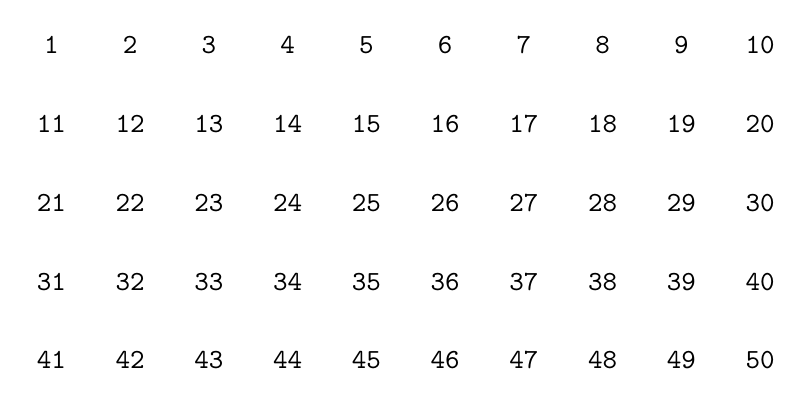
\begin{tikzpicture}
       \foreach \y in {0, 1, ..., 4}
       {
            \foreach \x in {1, 2, ..., 10}
            {
                \pgfmathtruncatemacro{\label}{(10*(4 - \y) + \x};
                \node at (\x, \y) { \tt \label };
            }
       }

    \end{tikzpicture}
    \end{figure}

\end{frame}

\begin{frame}[fragile]{Exemplo do crivo de Erastótenes para $N = 50$}

    \begin{figure}
    \centering
    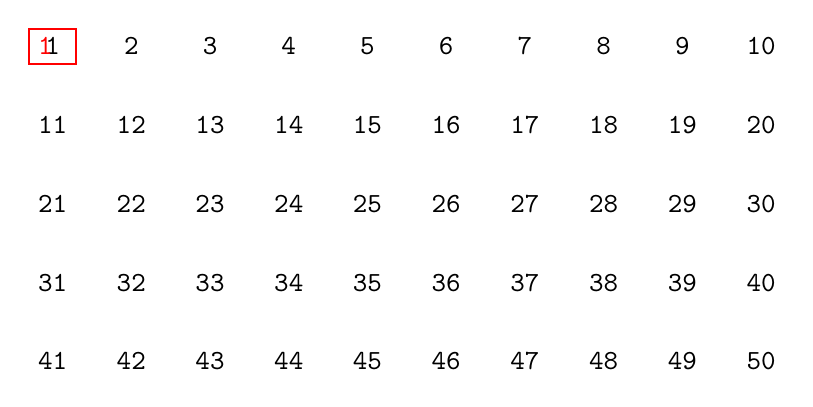
\begin{tikzpicture}
        \foreach \y in {0, 1, ..., 4}
        {
            \foreach \x in {1, 2, ..., 10}
            {
                \pgfmathtruncatemacro{\label}{(10*(4 - \y) + \x};
                \node at (\x, \y) { \tt \label };
            }
        }

        \foreach \n in { 1 }
        {
            \pgfmathtruncatemacro{\x}{\n - 10*round((\n - 1)/10)};
            \pgfmathtruncatemacro{\y}{4 - round((\n - 1)/10)};

            \node[draw, thick, red] at (\x, \y) {\tt \textcolor{red}{\n}};
        } 

    \end{tikzpicture}
    \end{figure}

\end{frame}

\begin{frame}[fragile]{Exemplo do crivo de Erastótenes para $N = 50$}

    \begin{figure}
    \centering
    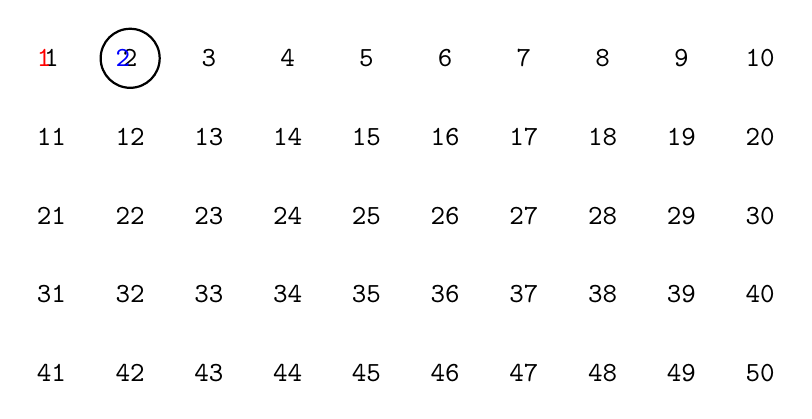
\begin{tikzpicture}
        \foreach \y in {0, 1, ..., 4}
        {
            \foreach \x in {1, 2, ..., 10}
            {
                \pgfmathtruncatemacro{\label}{(10*(4 - \y) + \x};
                \node at (\x, \y) { \tt \label };
            }
        }

        \foreach \n in { 1 }
        {
            \pgfmathtruncatemacro{\x}{\n - 10*round((\n - 1)/10)};
            \pgfmathtruncatemacro{\y}{4 - round((\n - 1)/10)};
            \node at (\x, \y) {\tt \textcolor{red}{\n}};
            %\node[draw, thick, red] at (\x, \y) {\tt \textcolor{red}{\n}};
        }

        \foreach \n in { 2 }
        {
            \pgfmathtruncatemacro{\x}{\n - 10*round((\n - 1)/10)};
            \pgfmathtruncatemacro{\y}{4 - round((\n - 1)/10)};
            \node[draw, circle, thick] at (\x, \y) {\tt \textcolor{blue}{\n}};
        }

    \end{tikzpicture}
    \end{figure}

\end{frame}

\begin{frame}[fragile]{Exemplo do crivo de Erastótenes para $N = 50$}

    \begin{figure}
    \centering
    \begin{tikzpicture}
        \foreach \y in {0, 1, ..., 4}
        {
            \foreach \x in {1, 2, ..., 10}
            {
                \pgfmathtruncatemacro{\label}{(10*(4 - \y) + \x};
                \node at (\x, \y) { \tt \label };
            }
        }

        \foreach \n in { 1 }
        {
            \pgfmathtruncatemacro{\x}{\n - 10*round((\n - 1)/10)};
            \pgfmathtruncatemacro{\y}{4 - round((\n - 1)/10)};
            \node at (\x, \y) {\tt \textcolor{red}{\n}};
        }

        \foreach \n in { 4, 6, ..., 50 }
        {
            \tikzmath{
                integer \k, \x;
                \k = (\n - 1)/10;
                \x = \n - 10*\k; 
                \y = 4 - \k; 
            }

            \node[draw, thick, red] at (\x, \y) {\tt \textcolor{red}{\n}};
        }

        \foreach \n in { 2 }
        {
            \pgfmathtruncatemacro{\x}{\n - 10*round((\n - 1)/10)};
            \pgfmathtruncatemacro{\y}{4 - round((\n - 1)/10)};
            \node[draw, circle, thick] at (\x, \y) {\tt \textcolor{blue}{\n}};
        }

    \end{tikzpicture}
    \end{figure}

\end{frame}

\begin{frame}[fragile]{Exemplo do crivo de Erastótenes para $N = 50$}

    \begin{figure}
    \centering
    \begin{tikzpicture}
        \foreach \y in {0, 1, ..., 4}
        {
            \foreach \x in {1, 2, ..., 10}
            {
                \pgfmathtruncatemacro{\label}{(10*(4 - \y) + \x};
                \node at (\x, \y) { \tt \label };
            }
        }

        \foreach \n in { 1 }
        {
            \pgfmathtruncatemacro{\x}{\n - 10*round((\n - 1)/10)};
            \pgfmathtruncatemacro{\y}{4 - round((\n - 1)/10)};
            \node at (\x, \y) {\tt \textcolor{red}{\n}};
        }

        \foreach \n in { 4, 6, ..., 50 }
        {
            \tikzmath{
                integer \k, \x;
                \k = (\n - 1)/10;
                \x = \n - 10*\k; 
                \y = 4 - \k; 
            }

            %\node[draw, thick, red] at (\x, \y) {\tt \textcolor{red}{\n}};
            \node at (\x, \y) {\tt \textcolor{red}{\n}};
        }

        \foreach \n in { 2, 3 }
        {
            \pgfmathtruncatemacro{\x}{\n - 10*round((\n - 1)/10)};
            \pgfmathtruncatemacro{\y}{4 - round((\n - 1)/10)};
            \node[draw, circle, thick] at (\x, \y) {\tt \textcolor{blue}{\n}};
        }

    \end{tikzpicture}
    \end{figure}

\end{frame}

\begin{frame}[fragile]{Exemplo do crivo de Erastótenes para $N = 50$}

    \begin{figure}
    \centering
    \begin{tikzpicture}
        \foreach \y in {0, 1, ..., 4}
        {
            \foreach \x in {1, 2, ..., 10}
            {
                \pgfmathtruncatemacro{\label}{(10*(4 - \y) + \x};
                \node at (\x, \y) { \tt \label };
            }
        }

        \foreach \n in { 1 }
        {
            \pgfmathtruncatemacro{\x}{\n - 10*round((\n - 1)/10)};
            \pgfmathtruncatemacro{\y}{4 - round((\n - 1)/10)};
            \node at (\x, \y) {\tt \textcolor{red}{\n}};
        }

        \foreach \n in { 4, 6, ..., 50 }
        {
            \tikzmath{
                integer \k, \x;
                \k = (\n - 1)/10;
                \x = \n - 10*\k; 
                \y = 4 - \k; 
            }

            \node at (\x, \y) {\tt \textcolor{red}{\n}};
        }

        \foreach \n in { 6, 9, ..., 50 }
        {
            \tikzmath{
                integer \k, \x;
                \k = (\n - 1)/10;
                \x = \n - 10*\k; 
                \y = 4 - \k; 
            }

            \node[draw, thick, red] at (\x, \y) {\tt \textcolor{red}{\n}};
        }


        \foreach \n in { 2, 3 }
        {
            \pgfmathtruncatemacro{\x}{\n - 10*round((\n - 1)/10)};
            \pgfmathtruncatemacro{\y}{4 - round((\n - 1)/10)};
            \node[draw, circle, thick] at (\x, \y) {\tt \textcolor{blue}{\n}};
        }

    \end{tikzpicture}
    \end{figure}

\end{frame}

\begin{frame}[fragile]{Exemplo do crivo de Erastótenes para $N = 50$}

    \begin{figure}
    \centering
    \begin{tikzpicture}
        \foreach \y in {0, 1, ..., 4}
        {
            \foreach \x in {1, 2, ..., 10}
            {
                \pgfmathtruncatemacro{\label}{(10*(4 - \y) + \x};
                \node at (\x, \y) { \tt \label };
            }
        }

        \foreach \n in { 1 }
        {
            \pgfmathtruncatemacro{\x}{\n - 10*round((\n - 1)/10)};
            \pgfmathtruncatemacro{\y}{4 - round((\n - 1)/10)};
            \node at (\x, \y) {\tt \textcolor{red}{\n}};
        }

        \foreach \n in { 4, 6, ..., 50 }
        {
            \tikzmath{
                integer \k, \x;
                \k = (\n - 1)/10;
                \x = \n - 10*\k; 
                \y = 4 - \k; 
            }

            \node at (\x, \y) {\tt \textcolor{red}{\n}};
        }

        \foreach \n in { 6, 9, ..., 50 }
        {
            \tikzmath{
                integer \k, \x;
                \k = (\n - 1)/10;
                \x = \n - 10*\k; 
                \y = 4 - \k; 
            }

            \node at (\x, \y) {\tt \textcolor{red}{\n}};
            %\node[draw, thick, red] at (\x, \y) {\tt \textcolor{red}{\n}};
        }


        \foreach \n in { 2, 3, 5 }
        {
            \pgfmathtruncatemacro{\x}{\n - 10*round((\n - 1)/10)};
            \pgfmathtruncatemacro{\y}{4 - round((\n - 1)/10)};
            \node[draw, circle, thick] at (\x, \y) {\tt \textcolor{blue}{\n}};
        }

    \end{tikzpicture}
    \end{figure}

\end{frame}

\begin{frame}[fragile]{Exemplo do crivo de Erastótenes para $N = 50$}

    \begin{figure}
    \centering
    \begin{tikzpicture}
        \foreach \y in {0, 1, ..., 4}
        {
            \foreach \x in {1, 2, ..., 10}
            {
                \pgfmathtruncatemacro{\label}{(10*(4 - \y) + \x};
                \node at (\x, \y) { \tt \label };
            }
        }

        \foreach \n in { 1 }
        {
            \pgfmathtruncatemacro{\x}{\n - 10*round((\n - 1)/10)};
            \pgfmathtruncatemacro{\y}{4 - round((\n - 1)/10)};
            \node at (\x, \y) {\tt \textcolor{red}{\n}};
        }

        \foreach \n in { 4, 6, ..., 50 }
        {
            \tikzmath{
                integer \k, \x;
                \k = (\n - 1)/10;
                \x = \n - 10*\k; 
                \y = 4 - \k; 
            }

            \node at (\x, \y) {\tt \textcolor{red}{\n}};
        }

        \foreach \n in { 6, 9, ..., 50 }
        {
            \tikzmath{
                integer \k, \x;
                \k = (\n - 1)/10;
                \x = \n - 10*\k; 
                \y = 4 - \k; 
            }

            \node at (\x, \y) {\tt \textcolor{red}{\n}};
        }

        \foreach \n in { 10, 15, ..., 50 }
        {
            \tikzmath{
                integer \k, \x;
                \k = (\n - 1)/10;
                \x = \n - 10*\k; 
                \y = 4 - \k; 
            }

            %\node at (\x, \y) {\tt \textcolor{red}{\n}};
            \node[draw, thick, red] at (\x, \y) {\tt \textcolor{red}{\n}};
        }


        \foreach \n in { 2, 3, 5 }
        {
            \pgfmathtruncatemacro{\x}{\n - 10*round((\n - 1)/10)};
            \pgfmathtruncatemacro{\y}{4 - round((\n - 1)/10)};
            \node[draw, circle, thick] at (\x, \y) {\tt \textcolor{blue}{\n}};
        }

    \end{tikzpicture}
    \end{figure}

\end{frame}

\begin{frame}[fragile]{Exemplo do crivo de Erastótenes para $N = 50$}

    \begin{figure}
    \centering
    \begin{tikzpicture}
        \foreach \y in {0, 1, ..., 4}
        {
            \foreach \x in {1, 2, ..., 10}
            {
                \pgfmathtruncatemacro{\label}{(10*(4 - \y) + \x};
                \node at (\x, \y) { \tt \label };
            }
        }

        \foreach \n in { 1 }
        {
            \pgfmathtruncatemacro{\x}{\n - 10*round((\n - 1)/10)};
            \pgfmathtruncatemacro{\y}{4 - round((\n - 1)/10)};
            \node at (\x, \y) {\tt \textcolor{red}{\n}};
        }

        \foreach \n in { 4, 6, ..., 50 }
        {
            \tikzmath{
                integer \k, \x;
                \k = (\n - 1)/10;
                \x = \n - 10*\k; 
                \y = 4 - \k; 
            }

            \node at (\x, \y) {\tt \textcolor{red}{\n}};
        }

        \foreach \n in { 6, 9, ..., 50 }
        {
            \tikzmath{
                integer \k, \x;
                \k = (\n - 1)/10;
                \x = \n - 10*\k; 
                \y = 4 - \k; 
            }

            \node at (\x, \y) {\tt \textcolor{red}{\n}};
        }

        \foreach \n in { 10, 15, ..., 50 }
        {
            \tikzmath{
                integer \k, \x;
                \k = (\n - 1)/10;
                \x = \n - 10*\k; 
                \y = 4 - \k; 
            }

            \node at (\x, \y) {\tt \textcolor{red}{\n}};
            %\node[draw, thick, red] at (\x, \y) {\tt \textcolor{red}{\n}};
        }


        \foreach \n in { 2, 3, 5, 7 }
        {
            \tikzmath{
                integer \k, \x;
                \k = (\n - 1)/10;
                \x = \n - 10*\k; 
                \y = 4 - \k; 
            }

            \node[draw, circle, thick] at (\x, \y) {\tt \textcolor{blue}{\n}};
        }

    \end{tikzpicture}
    \end{figure}

\end{frame}

\begin{frame}[fragile]{Exemplo do crivo de Erastótenes para $N = 50$}

    \begin{figure}
    \centering
    \begin{tikzpicture}
        \foreach \y in {0, 1, ..., 4}
        {
            \foreach \x in {1, 2, ..., 10}
            {
                \pgfmathtruncatemacro{\label}{(10*(4 - \y) + \x};
                \node at (\x, \y) { \tt \label };
            }
        }

        \foreach \n in { 1 }
        {
            \pgfmathtruncatemacro{\x}{\n - 10*round((\n - 1)/10)};
            \pgfmathtruncatemacro{\y}{4 - round((\n - 1)/10)};
            \node at (\x, \y) {\tt \textcolor{red}{\n}};
        }

        \foreach \n in { 4, 6, ..., 50 }
        {
            \tikzmath{
                integer \k, \x;
                \k = (\n - 1)/10;
                \x = \n - 10*\k; 
                \y = 4 - \k; 
            }

            \node at (\x, \y) {\tt \textcolor{red}{\n}};
        }

        \foreach \n in { 6, 9, ..., 50 }
        {
            \tikzmath{
                integer \k, \x;
                \k = (\n - 1)/10;
                \x = \n - 10*\k; 
                \y = 4 - \k; 
            }

            \node at (\x, \y) {\tt \textcolor{red}{\n}};
        }

        \foreach \n in { 10, 15, ..., 50 }
        {
            \tikzmath{
                integer \k, \x;
                \k = (\n - 1)/10;
                \x = \n - 10*\k; 
                \y = 4 - \k; 
            }

            \node at (\x, \y) {\tt \textcolor{red}{\n}};
            %\node[draw, thick, red] at (\x, \y) {\tt \textcolor{red}{\n}};
        }

        \foreach \n in { 14, 21, ..., 50 }
        {
            \tikzmath{
                integer \k, \x;
                \k = (\n - 1)/10;
                \x = \n - 10*\k; 
                \y = 4 - \k; 
            }

            \node[draw, thick, red] at (\x, \y) {\tt \textcolor{red}{\n}};
        }


        \foreach \n in { 2, 3, 5, 7 }
        {
            \tikzmath{
                integer \k, \x;
                \k = (\n - 1)/10;
                \x = \n - 10*\k; 
                \y = 4 - \k; 
            }

            \node[draw, circle, thick] at (\x, \y) {\tt \textcolor{blue}{\n}};
        }

    \end{tikzpicture}
    \end{figure}

\end{frame}
